\documentclass[aps,prd,twocolumn,showpacs,superscriptaddress,groupedaddress,nofootinbib]{revtex4}  % for review and submission
%\documentclass[aps,preprint,showpacs,superscriptaddress,groupedaddress]{revtex4}  % for double-spaced preprint
\usepackage{graphicx}  % needed for figures
\usepackage{dcolumn}   % needed for some tables
\usepackage{bm}        % for math
\usepackage{amsmath,amssymb}   % for math
\usepackage{color}
\usepackage{multirow}
\usepackage{aas_macros}
\usepackage{citesort}
%\usepackage{times}
\hyphenation{ALPGEN}
\hyphenation{EVTGEN}
\hyphenation{PYTHIA}
\newcommand{\mr}{\mathrm}
\newcommand{\mb}{\mathbf}
\renewcommand{\d}{\mathrm{d}}
\newcommand{\e}{\mathrm{e}}
\newcommand{\ii}{\mathrm{i}}
\newcommand{\bea}{\begin{eqnarray}}
\newcommand{\eea}{\end{eqnarray}}
\newcommand{\be}{\begin{equation}}
\newcommand{\ee}{\end{equation}}
\newcommand{\rund}[1]{\left(#1\right)}
\newcommand{\eck}[1]{\left[ #1 \right]}
\newcommand{\bigrund}[1]{\left{#1\right}}
\newcommand{\vc}[1]{\mbox{\boldmath $#1$}}
\newcommand{\dc}{\partial}
\newcommand{\msun}{h^{-1}M_{\odot}}

\def\llabel#1{\label{sc:#1}  {#1}\hspace{0.5cm}}
\def\elabel#1{\label{eq:#1}\fbox{#1}}
%\def\llabel#1{\label{sc:#1}}
%\def\elabel#1{\label{eq:#1}}

% avoids incorrect hyphenation, added Nov/08 by SSR
\hyphenation{ALPGEN}
\hyphenation{EVTGEN}
\hyphenation{PYTHIA}

\def\Mpc{{\rm Mpc}}

\begin{document}
% The following information is for internal review, please remove them for submission
\widetext
% the following line is for submission, including submission to the arXiv!!
%\hspace{5.2in} \mbox{Fermilab-Pub-04/xxx-E}

%\title{Reconstruction of the Cosmic Tidal Field}
\title{Cosmic Tidal Reconstruction}


\author{Hong-Ming Zhu}
\affiliation{Key Laboratory for Computational Astrophysics,
National Astronomical Observatories, Chinese Academy of Sciences,
20A Datun Road, Beijing 100012, China}
\affiliation{University of Chinese Academy of Sciences, Beijing 100049, China}

\author{Ue-Li Pen}
\affiliation{Canadian Institute for Theoretical Astrophysics, 60 St. George Street, Toronto, ON M5S 3H8, Canada}
\affiliation{Canadian Institute for Advanced Research, CIFAR Program in Gravitation and Cosmology, Toronto, ON M5G 1Z8, Canada}
\affiliation{Perimeter Institute for Theoretical Physics, 31 Caroline St. N., Waterloo, ON, N2L 2Y5, Canada}

\author{Yu Yu}
\affiliation{Key laboratory for research in galaxies and cosmology,
Shanghai Astronomical Observatory, Chinese Academy of Science,
80 Nandan Road, Shanghai 200030, China}

\author{Xinzhong Er}
\affiliation{Key Laboratory for Computational Astrophysics,
National Astronomical Observatories, Chinese Academy of Sciences,
20A Datun Road, Beijing 100012, China}
\affiliation{INAF, Osservatorio Astronomico di Roma, via Frascati 33, 
I-00040, Monteporzio Catone, Italy}

\author{Xuelei Chen}
\affiliation{Key Laboratory for Computational Astrophysics,
National Astronomical Observatories, Chinese Academy of Sciences,
20A Datun Road, Beijing 100012, China}
\affiliation{Center of High Energy Physics, Peking University, Beijing 100871, China}

\date{\today}

\begin{abstract}
The gravitational interaction of a long wavelength tidal field with
small scale density fluctuations leads to anisotropic distortions of the local 
%small scale matter 
two point correlation function.
Since the correlation function is statistically 
isotropic in the absence of tidal interactions, the tidal distortions
can be used to reconstruct the long wavelength tidal field in analogy with
CMB lensing.
In this paper we quantify how the optimal reconstrunction using these
tidal distortions.
The information encoded in the small scale structures enables accurate
reconstruction of the matter density field on large scales, 
$k\lesssim0.1h/\mr{Mpc}$.
We perform cosmic tidal reconstruction in $N$-body simulations and find the 
cross correlation coefficient between the reconstructed field and the original
density field is above 0.8 and close to 0.9 on some scales.
This allows the reconstruction of radial modes lost in 21cm intensity mapping
surveys.

%(old abstract)We provide a comprehensive illustration of cosmic tidal 
%reconstruction, including kinematics, dynamics, reconstruction algorithm and 
%tidal shear estimators. We study cosmic tidal reconstruction in $N$-body 
%simulations. 
%At last, we exmaine the validity of such method and discuss future applications.
\end{abstract}

\pacs{}
\maketitle
%\section{\label{sec:level1}First-level heading}
% sections are not used for PRL papers

\section{Introduction}
The large scale structure contains a wealth of information about our Universe.
The cosmic acceleration, neutrino masses, early universe models and  
other properties of the Universe can  be inferred with current or upcoming surveys.
Current data indicate a university with small Gaussian initial density perturbations. 
These grow due to gravitational interaction, nonlinearities develope and couplings 
between different modes were induced.
This leads to striking non-Gaussian features in the present large scale structure
of the Universe, limiting the cosmological information that can be extracted 
from galaxy surveys.
At the same time, however, such correlations between the different
perturbation modes on different scales also imply that we could infer information about the large scale  
density field by observing small scale density fluctuations.

The basic idea of such reconstruction is that the evolution of 
small scale density perturbations $\bm{k}_S$ are modulated by a long
wavelength perturbation $\bm{k}_L$, causing both isotropic and anisotropic
distortions of the local power spectrum \cite{2014:tidal}. 
The isotropic distortion, which depends only on the magnitude of the 
wavenumber $\bm{k}_S$, is mainly due to the change in the background density 
from the long wavelength density perturbation $\nabla^2\Phi_{L}\propto\delta_L$.
The anisotropic distortion, which also depends on the direction of $\bm{k}_S$,
is induced by the long wavelength tidal field 
$t_{ij}=\Phi_{L,ij}-\delta_{ij}\nabla^2\Phi_{L}/3$.
Using the isotropic modulation on the small scale power spectrum to recover
the large scale density field were studied in Ref.\cite{2014li}.
%\textcolor{blue}{ue-li can you add something about Bond's work here?
%I'm not very clear what they have done.}
However, the anisotropic distortions are more robust, since many other 
processes can also lead to isotropic distortions in the local small scale 
power spectrum. By applying quadratic estimators which quantify the local 
anisotropy of small scale filamentary structures, the long wavelength 
tidal field can be reconstructed accurately \cite{2012:pen}.
In general, this method can be applied to obtain measurement of long wavelength 
modes with better precision, this is especially valuable when these modes can not be 
obtained directly. 
The reconstruction of the long wavelength tidal field from the distorted local 
power spectrum is similar to the reconstruction of 
shear fields in gravitational lensing \cite{2008:lu,2010lu}.


In this paper we present the cosmic tidal reconstruction method in detail. 
%To get an intuitive understanding of the anisotropic distortions result from
%the tidal interaction, we first introduce the description of the deformation
%of a dark matter fluid element,  then we discuss the evolution of small scale 
%density fluctuations 
The evolution of small scale density fluctuations in the presence of the 
long wavelength tidal field $t_{ij}$ has been studied extensively in 
Ref.\cite{2014:tidal}.
The tidal distorted parts in the local small scale power spectrum is given by 
\begin{equation}
\delta P(\bm{k}_S,\tau)|_{t_{ij}}=
\hat{k}_S^i\hat{k}_S^jt_{ij}^{(0)}P_{1s}(k_S,\tau)f(k_S, k_L,\tau),
\end{equation}
where $\hat{\bm{k}}$ denotes the unit vector in the direction of $\bm{k}$,
$P_{1s}(k_S,\tau)$ is the isotropic linear power spectrum, 
$f(k_S, k_L, \tau)$ describes the coupling of the long wavelength tidal field 
to the small scale density fluctuations and superscript $(0)$ denotes some 
``initial'' time. 
%If we make a decomposition in the line of sight (l.o.s.) direction,  
%the anisotropic (traceless) tidal field tensor $t_{ij}$ can be written in the following form:
The anisotropic distortion can be decomposed into several orthogonal quadrupolar
distortions if we write $t_{ij}$ in the following form:
\begin{eqnarray}
t_{ij}=\left( \begin{array}{ccc}
\gamma_{1}-\gamma_{z} & \gamma_{2} & \gamma_{x}\\
\gamma_{2} & -\gamma_{1}-\gamma_{z} & \gamma_{y}\\
\gamma_{x} & \gamma_{y} & 2\gamma_z
\end{array} \right).
\label{eqn:tidalshear}
\end{eqnarray}
While (\ref{eqn:tidalshear}) in principle has 6 independently observable components,
we will be focussing on  the
two transverse shear terms 
$(\hat{k}_1^2-\hat{k}_2^2)\gamma_1^{(0)}P_{1s}f$
and $2\hat{k}_1\hat{k}_2\gamma_2^{(0)}P_{1s}f$, which 
describe orthogonal quadrupolar distortions in the tangential plane perpendicular 
to the line of sight.  The quadrupolar distortions containing $\hat{k}_3$
will be affected by peculiar velocities, and require additional treatments beyond the
scope of this paper.
Here $\gamma_{+}=(\Phi_{L,11}-\Phi_{L,22})/2$ and $\gamma_{\times}=\Phi_{L,12}$.
These two tidal shear fields can be converted into the 2D convergence field
$\kappa_\mr{2D}=(\Phi_{L,11}+\Phi_{L,22})/2$ 
using $\kappa_{\mr{2D},11}+\kappa_{\mr{2D},22}=
\gamma_{+,11}-\gamma_{+,22}+2\gamma_{\times,12}$.
We can obtain the 3D convergence field $\kappa_\mr{3D}=\nabla^2\Phi_L/3$ from 
$\kappa_\mr{3D,11}+\kappa_\mr{3D,22}=2\nabla^2\kappa_\mr{2D}/3$. 
The large scale density field $\delta_L$ is given by the 3D convergence field 
through the Poisson equation.
Here the two tidal shear fields are evaluated by applying
quadratic estimators to the density field as in weak lensing.
The optimal tidal shear estimators can be derived under the Gaussian assumption.

We call this method {\it cosmic tidal reconstruction}, as it exploits the
local tidal distorted anisotropic features.
Each independent measurement of the small scale power spectrum gives some 
information about the power spectrum on longer linear scales. 
%There are a lot of such measurements we can exploit on small scales, which provide little additional information in previous. 
Thus instead of being limited by the non-Gaussianity on small scales, we exploit these strong correlations to
improve the measurement of the large scale structure. 

Since we only use the tidal shear fields in the $x-y$ plane to reconstruct
the long wavelength density field, the change of long wavelength density
field $\delta_L$ along $z$ axis is inferred from the variations of tidal shear
fields $\gamma_1$ and $\gamma_2$ along $z$ axis.
We can not capture rapid changes of the density field along $z$ axis, 
i.e. those modes with large $k_\parallel$.
The noise of the reconstructed mode $\kappa_\mr{3D}(\bm{k})$ is 
\begin{eqnarray}
\sigma^2_{\kappa_\mr{3D}}\propto\bigg(\frac{k^2}{k_\perp^2}\bigg)^2,
\end{eqnarray}
where the anisotropic dependence is due to we only use $\gamma_{1}$ and 
$\gamma_2$ to reconstruct the large scale density field. 
The noise is infinite when $k_\perp\to0$. 
In this case, we expect these modes contain nothing but noise. 
The well reconstructed modes are those with small $k_\parallel$ and large
$k_\perp$. This helps the correlation of 21cm intensity mapping survey with
other cosmic probes, including ISW, lensing, photo-z, optical depth,
and others.  These low  $k_\parallel$ are normally lost in the
foreground subtraction process \cite{2007ApJ...660.1030F,2008MNRAS.384..291A}.

%... \textcolor{blue}{ue-li can you add something here?}

The local quadrupolar distortions have also been discussed in
\cite{masui2010,2012:jeong}
%\textcolor{blue}{ue-li can you also add something here?}
where the theoretical constructions were outlined.  This paper expands
on the early work by considering puirely transverse reconstructions.

%In Table I, we summarize the notations we adopted in this paper.
The remaining part of this paper is organized as follows.
In Section II, we present the basic formalism, including kinematics, 
dynamics, reconstruction algorithm and tidal shear estimators. In Section III,
we study cosmic tides in $N$-body simulations. In Section IV,
we examine the validity of cosmic tidal reconstruction and discuss its 
future applications.

\section{Tidal deformation}

The motion of a dark matter fluid element in the Universe includes 
translation, rotation and deformation. 
Let us consider two neighboring points $P_0$ 
and $P$ in the fluid at time $t_0$, the velocity  
$\bm{v}|_{P}$ can be expanded as
%\begin{eqnarray}
%v^i|_{P}=v^i|_{P_0}+v^i_{\ ,j}|_{P_0}\Delta x^j,
%\end{eqnarray}
%where $v^i_{\ ,j}=\partial v^i/\partial x^j$ is the velocity gradient tensor.
\begin{eqnarray}
v^i|_{P}=v^i|_{P_0}+(S^i_{\ j}+A^i_{\ j})|_{P_0}\Delta x^j.
\end{eqnarray}
where the symmetric part $S^i_{\ j}=(v^i_{\ ,j}+v_j^{\ ,i})/2$  is the deformation velocity tensor in fluid 
mechanics, with diagonal components describing the stretching along three
axises and off-diagonal components describing the shear motion;
the anti-symmetry part $A^i_{\ j}=(v^i_{\ ,j}-v_j^{\ ,i})/2$ describes the rotation of this fluid element.
In the free falling reference system of this fluid element, $v|_{P_0}=0$.
Neglecting the rotation,  the position of $P$ at time $t$ is given by 
\begin{eqnarray}
\Delta x^i(t)|_P=\Delta x^i_0+\int_{t_0}^tS^i_{\ j}(t{'})|_{P_0}dt{'}  \Delta x_0^j,
\end{eqnarray}
where $\Delta x_0^i$ is the initial separation between $P_0$ and $P$.
The shape tensor $\mathfrak{S}^i_{\ j}=\int_{t_0}^tS^i_{\ j}(t{'})|_{P_0}dt{'}$ 
describes the deformation. 
In the local inertial frame, the free falling dark matter fluid elements 
are only sensitive to the residual gravitational forces, similar to the 
ocean tides on Earth induced by the tidal forces from the Moon and the Sun.
We call such effects by the surrounding large scale structure {\it cosmic tides}.  
The observable structures of baryonic tracers
 will also exhibit the same local anisotropies. The long wavelength tidal field and the 
large scale density may then be inferred from observation. In reality, the 
interaction between the long wavelength tidal field
and small scale density fluctuations is more complicated than the displacement 
of particles in a fluid element, we shall discuss this in more detail below. 
%There is also anisotropic deformation induced by local structure, 
%which would be a source of noise for tidal reconstruction. Such noise can be reduced
%by Gaussianization procedure, e.g. the logarithmic transformation\cite{2012:log}), we shall discuss this 
%in the section on tidal reconstruction.  
%==========================


%In this subsection, we will study the effect of a long wavelength tidal field
%on the evolution of small scale density perturbations, assuming $k_L\ll k_S$. 
%We foucus on the residual anisotropic gravitational interaction, i.e. the 
%effect seen by an observer in the local free falling frame. 
%Such tidal interaction has been studied extensively in \cite{2014:tidal},
%we will mostly follow their calculations with emphasis on reducing small scale
%non-Gaussianities by a logarithmic transform \cite{2012:log}.
%In this paper we will foucus on the effect of the traceless tidal field 
%$t_{ij}=\Phi_{L,ij}-\delta_{ij}\nabla^2\Phi_{L}/3$ as the change of shape is 
%more robust while many other processes can lead to a change of number density.

In the expanding universe, the equation of motion for a particle is 
\begin{equation}
\label{eq1}
\frac{d^2{\bm x}}{d\tau}+\mathcal{H}(\tau)\frac{d{\bm x}}{d\tau}
=-\nabla_{\bm x}\phi,
\end{equation}
where $\bm{x}$ is the comoving Eulerian coordinate, $\tau$ is the conformal 
time, $\mathcal{H}=d\mr{ln}a(\tau)/d\tau$ is the comoving Hubble parameter, 
$a(\tau)$ is the scale factor and $\phi$ is the gravitational potential.
In Lagrangian perturbation theory, the dynamical variable is the Lagrangian 
displacement field $\mathbf{s}(\bm{q},\tau)$, defined as
\begin{equation}
\label{eq2}
\bm{x}(\tau)=\bm{q}+\mb{s}(\bm{q},\tau),
\end{equation}
where $\bm{q}$ is the comoving Lagrangian coordinate. The displacement field
maps the initial particle position $\bm{q}$ into the final Eulerian position
$\bm{x}$.
The density contrast $\delta(\bm{x})$ is given by the mass conservation relation:
\begin{eqnarray}
\label{eq3}
\delta(\bm{x}(\bm{q},\tau))=\mr{det}(\delta^i_{\ j}+\mr{M}^i_{\ j}
(\bm{q},\tau))-1
\end{eqnarray}
where $\mr{M}^i_{\ j}=\partial\mr{s}^i/\partial q^j$.
% and
%\begin{equation}
%\frac{\partial}{\partial q^i}=\frac{\partial}{\partial x^i}+\mr{M}^j_{\ i}\frac{\partial}{\partial x^j}.
%\end{equation}

To study the evolution of small scale density perturbations  
in the presence of the long wavelength tidal field, we decompose the gravitational 
potential $\phi$  into a part sourced by the small scale density fluctuations, 
$\Phi_s$ and a part induced by the long wavelength tidal field up to second order,
%\cite{2014:tidal}, i.e. 
\begin{eqnarray}
\label{eq4}
\phi(\bm{x}(\bm{q},\tau))=\Phi_s(\bm{x}(\bm{q},\tau))
+\frac{1}{2}t_{kl}(\bm{0}, \tau)x^k x^l + ...
\end{eqnarray}
The tidal field can be written as $t_{ij}(\bm{0}, \tau)=T(\tau)t_{ij}^{(0)}(\bm{0})$, 
where superscript  $(0)$ denotes the tidal field evaluated at the ``initial'' time $\tau_0$,
$T(\tau)=D(\tau)/a(\tau)$ is the transfer function, which is independent of wavelength 
during the linear growth stage,  $D(\tau)$ is the linear growth function, $D(\tau_0)=a(\tau_0)=1$.
Note that at the origin of the free falling frame, the contribution from the tidal 
field is by definition zero. The small scale potential $\Phi_s$ satisfies the Poisson equation,
\begin{eqnarray}
\label{eq5}
\nabla^2\Phi_s=4\pi Ga^2\bar{\rho}\delta=
\frac{3}{2}\Omega_m(\tau)\mathcal{H}^2\delta,
\end{eqnarray}
where $\Omega_m(\tau)$ is the density parameter at $\tau$.

The above equations could be solved perturbatively.
We decompose the displacement as
\begin{eqnarray}
\mb{s}=\mb{s}_s+\mb{s}_t,
\end{eqnarray}
where $\mb{s}_s$ and $\mb{s}_t$ are the contributions from the small scale local potential
and long wavelength tidal field respectively. Then 
$\mr{M}^i_{\ j}=\mr{M}^{\ i}_{s\ j}+\mr{M}^{\ i}_{t\ j}$ with
$\mr{M}^{\ i}_{s\ j}=\partial \mr{s}_s^i/\partial q^j$,
$\mr{M}^{\ i}_{t\ j}=\partial \mr{s}_t^i/\partial q^j$. 
Here we only consider
the linear displacement $\mb{s}_{1s}$, $\mb{s}_{1t}$ and the quadratic term 
$\mb{s}_{2t}$ from the coupling of $\mb{s}_{1s}$ and $\mb{s}_{1t}$, and neglect
the terms of order $(\mb{s}_{1s})^2$, which are 
nonlinear interaction between small scale modes.
In the follow calculations, we focus on the coupling between the long mode 
(large scale tidal field) and the short mode (small scale density field), 
assuming that both large and small scale density fields underwent linear evolutions.

At linear order, Eq.(\ref{eq1}) becomes two equations for 
$\mb{s}_{1s}$ and $\mb{s}_{1t}$, respectively,
\begin{eqnarray}
\left[\frac{d^2}{d\tau^2}+\mathcal{H}\frac{d}{d\tau}\right]\mr{s}_{1s}^i(\bm{q},\tau)&=&
-{\partial}_q^i\Phi_{1s}(\bm{q},\tau),\nonumber\\
\left[\frac{d^2}{d\tau^2}+
\mathcal{H}\frac{d}{d\tau}\right]\mr{s}_{1t}^i(\bm{q},\tau)&=&
-\frac{1}{2}{\partial}^i_q[t_{kl}(\tau)q^kq^l], 
\end{eqnarray}
where $\partial_q^i \equiv\delta^{ij}\partial/\partial q^j$, and 
$\nabla_q^2\Phi_{1s}=3\Omega_m(\tau)\mathcal{H}^2\delta_{1s}/2$,
$\delta_{1s}=-\mr{s}_{1s,i}^{\ i}$. \textcolor{red}{Should add more detail here.}

The first equation can be solved to get 
\begin{eqnarray}
\mr{s}_{1s}^i(\bm{q},\tau)
=-\frac{\partial^i_q}{\nabla^2_q}\delta_{1s}(\bm{q},\tau)
=-D(\tau)\frac{\partial^i_q}{\nabla^2_q}\delta_{1s}(\bm{q},\tau_0).
\end{eqnarray}
where we use $\frac{1}{\nabla^2}$ to denote the inverse operator for $\nabla^2$, which 
can be easily computed in Fourier space. 
The second equation which describes the evolution of the displacement induced 
by the long wavelength tidal field can be integrated to get 
\begin{eqnarray}
\mr{s}_{1t}^i(\bm{q},\tau)=-F(\tau)t^{(0)i}_{\ \ \ \ j}q^j,
\end{eqnarray}
where 
%\begin{eqnarray}
%F(\tau)=\int_0^\tau\frac{d\tau{'}}{a(\tau{'})}\int_0^{\tau{'}}
%d\tau{''}a(\tau{''})T(\tau{''}).
%\end{eqnarray}
\begin{eqnarray}
F(\tau)=\int_0^\tau{d\tau{''}}{a(\tau{''})}T(\tau'')G(\tau-\tau'')
\end{eqnarray}
and $G(\tau-\tau'')=\int^\tau_{\tau''}d\tau'/a(\tau')$.
The induced linear density fluctuation $\delta_{1t}$ is given by
\begin{eqnarray}
\delta_{1t} = -\mr{s}^{\ i}_{1t,i} = F(\tau)t^{(0)i}_{\ \ \ \ i}.
\end{eqnarray}
The trace of the tidal field $t_{ij}$ is zero, i.e. $\delta_{1t}=0$, 
so there is no first order contribution to the density from the tidal field.

The evolution equation for $\mb{s}_{2t}$ involves quadratic mixed terms from
the coulping between $\mb{s}_{1s}$ and $\mb{s}_{1t}$. Inserting the Poisson 
equation\footnote{Note here at linear order $\mr{tr}\mr{M}_{1t}=-\delta_{1t}$
should not be included when expanding Eq.(\ref{eq5}), as it is induced by the 
long wavelength tidal field $t_{ij}$, while the coupling between $\mr{M}_{1s}$ 
and $\mr{M}_{1t}$ should be included when expanding to second order as they 
source the local gravitational potential $\Phi_s$.}
to Eq.(\ref{eq1}), and subtracting the evolution equations for $\mb{s}_{1s}$,
$\mb{s}_{1t}$ and $\mb{s}_{2s}$ leads to
\begin{eqnarray}
\label{eq18}
&&\frac{d^2}{d\tau^2}\sigma_{2t}+\mathcal{H}\frac{d}{d\tau}\sigma_{2t}-
\frac{3}{2}\Omega_m(\tau)\mathcal{H}^2\sigma_{2t} \nonumber \\
&=&-\frac{3}{2}\Omega_m(\tau)\mathcal{H}^2
\delta_{1s}\delta_{1t}
%\bigg|_{\bm{q},\tau}
+\bigg(\frac{\partial^i\partial^j}{\nabla^2}\delta_{1s}\bigg)
%\bigg|_{\bm{q},\tau}
t_{ij}(\tau),
\end{eqnarray}
where $\sigma\equiv\mr{s}^i_{\ ,i}$.
The first term on the right hand of Eq.(\ref{eq18}) vanishes since 
$\delta_{1t}=0$.
This equation can be solved numerically to get 
\begin{eqnarray}
\sigma_{2t}(\bm{q},\tau)=D_{\sigma1}(\tau)
\bigg(\frac{\partial^i\partial^j}{\nabla^2}\delta_{1s}(\bm{q},\tau)
\bigg)t_{ij}^{(0)},
\end{eqnarray}
where
\begin{eqnarray}
D_{\sigma1}(\tau)=
%\frac{1}{D(\tau)}
\int^\tau_0d\tau'
\frac{H(\tau)D(\tau')-H(\tau')D(\tau)}{\dot{H}(\tau')D(\tau')-
H(\tau')\dot{D}(\tau')}\frac{D^2(\tau')}{D(\tau)a(\tau')}.
\end{eqnarray}

The difference between density contrasts with and without $t_{ij}$ at $\bm{x}$ 
is 
\begin{eqnarray}
\delta_{t}(\bm{x})=\delta(\bm{x})-\delta(\bm{x})|_{t_{ij}=0}.
\end{eqnarray}
Since the tidal field induces the displacement $\mb{s}_{t}$ 
in addition to $\mb{s}_{s}$, the same Lagrangian coordinate $\bm{q}$ corresponds
to different $\bm{x}$ in these two cases. In the presence of $t_{ij}$, 
$\bm{x}=\bm{q}+\mb{s}_{1s}+\mb{s}_{1t}$. Here $\delta_{1s}$ solved from
linear equations gives the density at 
$\bm{x}_s=\bm{q}+\mb{s}_{1s}=\bm{x}-\mb{s}_{1t}$.
Taking this into account and using Eq.(\ref{eq3}), one finally get 
\begin{eqnarray}
\delta_t(\bm{x},\tau)=\delta_{1t}(\bm{x})-\sigma_{2t}(\bm{x})+
\delta_{1t}(x)\delta_{1s}(\bm{x}) \nonumber \\
+\mr{tr}(\mr{M}_{1s}\mr{M}_{1t})|_{\bm{x}}
-s^i_{1t}\partial_i \delta_{1s}(\bm{x}).
\end{eqnarray}
Inserting first and second order solutions and noting that the tidal field
is traceless, we obtain the anisotropic small scale
density fluctuations induced by  long wavelength tidal field $t_{ij}$:
\begin{eqnarray}
\label{eq22}
\delta_t(\bm{x},\tau)=t^{(0)}_{ij}\bigg[
\alpha(\tau)\frac{\partial^i\partial^j}{\nabla^2}+\beta(\tau)x^i\partial^j
\bigg]\delta_{1s}(\bm{x},\tau),
\end{eqnarray}
where $\alpha(\tau)=-D_{\sigma1}(\tau)+F(\tau)$ and $\beta(\tau)=F(\tau)$.

In the above we have used the linear density-displacement relation 
$\delta_{1s}=-s_{1s,i}^{\ i}$  to derive the small scale density field $\delta_{1s}$ 
from the linear displacement field $\bm{s}_{1s}$. However,
this linear relation does not hold well at low redshifts and small scales
\cite{2012:log}. Improvement can be made by adopting the better held 
logarithmic relation between the divergence
of the displacement field and the density field  \cite{2012:log},
\begin{eqnarray}
s_{1s,i}^{\ i} = -\mr{ln}(1+\delta_{1s})+\langle\mr{ln}(1+\delta_{1s})\rangle,
\end{eqnarray}
Below we will use the logarithmic variable $\delta_g=\mr{ln}(1+\delta_{1s})$ in 
place of $\delta_{1s}$ in the reconstruction. This
logarithmic transformation reduces non-Gaussianities in the evolved density field, hence 
improves the reconstruction \cite{2012:pen}. 

%Here we consider the squeezed limit, i.e. the tidal field $t_{ij}$ can be taken
%as constant in a small patch
The tidal field $t_{ij}$ with wavenumber $k_L$ can be taken as constant in a 
small patch with scale $\ll1/k_L$. Note it is different to 
have a constant tidal field $t_{ij}$ and a contant gravitational field $\Phi_L$.
The former corresponds to the second spatial derivative of the latter.
The local correlation function in the free falling frame is 
\begin{eqnarray}
\xi(\bm{r},\tau)=\langle\delta(\bm{0},\tau)\delta(\bm{r},\tau)\rangle,
\end{eqnarray}
where $\delta=\delta_{1s}+\delta_{t}$. Using Eq.(\ref{eq22}), we obtain
\begin{eqnarray}
\label{eq25}
\xi(\bm{r},\tau)&=&\xi_{1s}(r,\tau)\nonumber\\
&+&t_{ij}^{(0)}\bigg[2\alpha(\tau)\frac{\partial^i\partial^j}{\nabla^2}+
\beta(\tau)r^i\partial^j\bigg]\xi_{1s}(r,\tau),
\end{eqnarray}
where $\xi_{1s}(r,\tau)=\langle\delta_{1s}(\bm{0},\tau)
\delta_{1s}(\bm{r},\tau)\rangle$ is the isotropic linear matter correlation
function. 
The anisotropic distortion of the locally measured small scale density 
correlation function is induced by the long wavelength tidal field $t_{ij}$.
%The large scale tidal field $t_{ij}$ leads to a local anisotropy 
%of quadratic statistics.
Transform Eq.(\ref{eq25}) to Fourier space, we will get the local tidal distorted
power spectrum. We abbreviate $k_S$ as $k$ and suppress the 
argument $k_L$ since $T(\tau)$ is scale independent, then we finally obtain
\begin{equation}
\label{eq26}
P(\bm{k},\tau)|_{t_{ij}}=P_{1s}(k,\tau)+
\hat{k}^i\hat{k}^jt_{ij}^{(0)}P_{1s}(k,\tau)f(k,\tau),
\end{equation}
where $P_{1s}(k,\tau)$ is the undistorted small scale power spectrum, and
\begin{equation}
f(k,\tau)=2\alpha(\tau)-\beta(\tau){d\mr{ln}P_{1s}(k,\tau)}/{d\mr{ln}k}.
\end{equation}
%Thus we can exploit the anisotropy statistics of small scale density distribution
% to reconstruct the long wavelength tidal field 
%$t_{ij}$ using estimators quadratic in $\delta_g$ \cite{2012:pen}. By 
%combining different parts of the traceless tidal tensor field, we get an 
%estimate of the trace of the tensor $\Phi_{L,ij}$, which corresponds to the 
%large scale density field $\delta_L$. The reconstruction of the tidal field 
%$t_{ij}$ is almost the same as weak lensing reconstruction, especially the 
%21cm lensing \cite{2008:lu,2010lu}.
%=============================

\section{Tidal Reconstruction}
In this section we first obtain the tidal shear estimators,  then 
present the algorithm for density reconstruction.

\subsection{Tidal Shear Estimators}
The long wavelength tidal field can be considered as constant if the coherence scale 
of the small scale density field is much smaller 
than that of the long wavelength tidal field.
We first consider the long wavelength limit, where $\gamma_+$ and 
$\gamma_\times$ are constant in space, then generalize the estimators to the 
spatial varying case. We also discuss what happens when the long wavelength 
limit does not hold.

Given the tidal distortion on power spectrum (Eq.\ref{eq26}), in the long wavelength limit and under the Gaussian assumption, 
quadratic shear estimators can be constructed either by using the maximum likelihood method\cite{2008:lu}
or the inverse variance weighting from galaxy density contrast $\delta_g$ 
\cite{2010lu,2012bucher}:
\begin{equation}
\hat{\gamma}_+=\frac{1}{Q_{\gamma_+}}\int\frac{d^3k}{(2\pi L)^3}
|{\delta}_g(\bm{k})|^2
\frac{P(k,\tau)}{P_{\mr{tot}}^2(k,\tau)}f(k,\tau)(\hat{k}_1^2-\hat{k}_2^2),
\end{equation}
\begin{equation}
\hat{\gamma}_\times=\frac{1}{Q_{\gamma_\times}}\int\frac{d^3k}{(2\pi L)^3}
|{\delta}_g(\bm{k})|^2
\frac{P(k,\tau)}{P_{\mr{tot}}^2(k,\tau)}f(k,\tau)(2\hat{k}_1\hat{k}_2),
\end{equation}
where $P_\mr{tot}(k)=P(k)+P_\mr{N}(k)$ is the observed matter \textcolor{red}{galaxy?} power spectrum, and
\begin{eqnarray}
Q_{\gamma_+}=\int\frac{d^3k}{(2\pi)^3}
\frac{P^2(k,\tau)}{P_{\mr{tot}}^2(k,\tau)}f^2(k,\tau)(\hat{k}_1^2-\hat{k}_2^2)^2,
\end{eqnarray}
%and
%\begin{eqnarray}
%\hat{\gamma}_\times=\frac{1}{Q_{\gamma_\times}}\int\frac{d^3k}{(2\pi)^3}
%|{\delta}_g(\bm{k})|^2L^{-3}
%%\nonumber\\&&\times
%\frac{P(k,\tau)}{P_{\mr{tot}}^2(k,\tau)}
%%\bigg[2\alpha-\beta\frac{d\mr{ln}P(k)}{d\mr{ln}k}\bigg]
%f(k,\tau)
%(2\hat{k}_1\hat{k}_2),
%\end{eqnarray}
%where
\begin{eqnarray}
Q_{\gamma_\times}=\int\frac{d^3k}{(2\pi)^3}
\frac{P^2(k,\tau)}{P_{\mr{tot}}^2(k,\tau)}
%\bigg[2\alpha-\beta\frac{d\mr{ln}P(k)}{d\mr{ln}k}\bigg]^2
f^2(k,\tau)
(2\hat{k}_1\hat{k}_2)^2.
\end{eqnarray}
After integrating over angles in Fourier space, we have
\begin{equation}
Q_{\gamma_+}=Q_{\gamma_\times}=Q=\int\frac{2k^2dk}{15\pi^2}\frac{P^2(k,\tau)}{P_{\mr{tot}}^2(k,\tau)}
%\bigg[2\alpha-\beta\frac{d\mr{ln}P(k)}{d\mr{ln}k}\bigg]^2
f^2(k,\tau)
\label{eq:Q}
\end{equation}
Using Parseval's theorem, we can rewrite the  above equations in real space,
\begin{eqnarray}
\label{eq36}
\hat{\gamma}_+=\frac{1}{L^3}\int\d^3x
\big[{\delta}^{w_1}_g(\bm{x}){\delta}^{w_1}_g(\bm{x})-
{\delta}^{w_2}_g(\bm{x}){\delta}^{w_2}_g(\bm{x})\big],
\end{eqnarray}
and
\begin{eqnarray}
\label{eq37}
\hat{\gamma}_\times=\frac{1}{L^3}\int\d^3x
\big[2{\delta}^{w_1}_g(\bm{x}){\delta}^{w_2}_g(\bm{x})\big],
\end{eqnarray}
where ${\delta}^{w_1}_g(\bm{x})$ and ${\delta}^{w_2}_g(\bm{x})$ 
are two filtered density fields. In Fourier space, they are given by
\begin{eqnarray}
{\delta}_g^{w_i}(\bm{k})=\delta_g(\bm{k})w_i(\bm{k}),
\end{eqnarray}
where 
\begin{eqnarray}
\label{eq:filter}
w_i(\bm{k})=\sqrt{\frac{P(k,\tau)}{QP^2_\mr{tot}(k,\tau)}}
%\bigg[2\alpha-\beta\frac{d\mr{ln}P(k)}{d\mr{ln}k}\bigg]^{1/2}
f(k,\tau)^{1/2}
\hat{k}_i.
\end{eqnarray}


In deriving Eq.(\ref{eq36}) and Eq.(\ref{eq37}), we have assumed that the tidal 
shear field is constant in space. 
From the expressions for $\hat{\gamma}_+$ and $\hat{\gamma}_\times$, we can 
see the terms in square brackets give estimates for $\gamma_+$ and 
$\gamma_\times$ at $\bm{x}$, while the integral $\int d^3x/L^3$ averages the 
local value over the whole space $L^3$.
If the fluctuation of the tidal field $t_{ij}$ changed on a larger scale than the filtering scale, 
we can use the localized estimation in the square brackets as estimates
for $\gamma_{+,\times}$ \cite{2008:lu,2010lu,2012bucher}. 
The unbiased minimum variance 
estimates of the spatial varying tidal field in the long wavelength limit is given by
\begin{eqnarray}
\label{eq40}
\hat{\gamma}_+(\bm{x})&=&
\big[{\delta}^{w_1}_g(\bm{x}){\delta}^{w_1}_g(\bm{x})-
{\delta}^{w_2}_g(\bm{x}){\delta}^{w_2}_g(\bm{x})\big],\nonumber\\
\hat{\gamma}_\times(\bm{x})&=&
\big[2{\delta}^{w_1}_g(\bm{x}){\delta}^{w_2}_g(\bm{x})\big].
\end{eqnarray}

The estimators given in Eq.(\ref{eq40}) were derived assuming that compared with the small scale density field, the long wavelength tidal shear fields vary slowly.  If this long wavelength 
limit is not satisfied, the tidal shear reconstruction would be biased by a 
multiplicative bias factor $b(\bm{k})$, which approaches to unity in the limit
$k\to0$ and decreases when $k$ increases \cite{2008:lu,2012bucher}. 
%The bias factor can derived in the case of Gaussian density fluctuations
%\cite{2008:lu}. It has also been studied numerically in CMB 
%lensing \cite{2012bucher}.
In the cosmic tidal reconstruction, we mainly use the nonlinear structures 
around the scale $1.25\ \mr{Mpc}/h$ to reconstruct the long wavelength tidal 
field \cite{2012:pen}, so for the reconstructed large scale density 
perturbations with wavenumber $k_L\lesssim0.1\ h$/Mpc we can ignore this 
multiplicative bias. 

\subsection{Density Reconstruction Algorithm}
The tensor field $\Phi_{L,ij}$ has six components. Such symmetric
$3\times3$ tensor can be decomposed into 6 orthogonal components 
\cite{1973gw,2012:jeong}, 
i.e. $\Phi_{L,ij}=A_a\epsilon^a_{ij}$, where $A_a$ is
the expansion coefficient and $\epsilon^a_{ij}$ statisfies the orthogonal
relation $\epsilon^a_{ij}\epsilon^{bji}\propto\delta^{ab}$. We decompose
$\Phi_{L,ij}$ as
\begin{eqnarray}
\Phi_{L,ij}
&=&(1+\epsilon_0)\delta_{ij}+t_{ij},
\end{eqnarray}
where $\epsilon_0=\nabla^2\Phi_L/3$, $\gamma_{+}=(\Phi_{L,11}-\Phi_{L,22})/2$,
$\gamma_{\times}=\Phi_{L,12}$, $\epsilon_{x}=\Phi_{L,13}$, 
$\epsilon_{y}=\Phi_{L,23}$, and 
$\epsilon_{z}=(2\Phi_{L,33}-\Phi_{L,11}-\Phi_{L,22})/6$. 
Here the tensor is decomposed in a way such that when reduced 
to the 2D case, notations reduce to those used in gravitational lensing, 
so the $z$ axis plays a different role than the $x-$ and $y-$axes.
For intuitive unsterdandings of these abstract symbols, 
see the figures in \cite{2012:jeong}. All these 6 different components will induce
different observable effects in the local quadratic statistics, including the
isotropic modulations ($\epsilon_0$) and anisotropic parts ($\gamma_+$, 
$\gamma_\times$, etc). The large scale gravitational potential $\Phi_L$ 
 is a single number, so it is six fold overdetermined. 
 %Using the isotropic modulation on small scale power specturm to recover
%the large scale density field (super sample signal) has been studied in
%\cite{2014li}. 
Li et al.\cite{2014li} used the isotropic modulation to reconstruct the large
scale density field. Here we focus on the ``change of shape", i.e. the traceless tidal field 
$t_{ij}=\Phi_{L,ij}-\nabla^2\Phi_{L}\delta_{ij}/3$ instead.
%through the relation 
%$\nabla^2\Phi_L=3K_{ij}t_{ij}/2$, where $K_{ij}=\partial_i\partial_j/\nabla^2$.
%where $\epsilon_0=(\psi_{,11}+\psi_{,22}+\psi_{,33})/3$ represents an isotropic
%modulation of the fluid element, $\gamma_{+}=(\psi_{,11}-\psi_{,22})/2$ and 
%$\gamma_{\times}=\psi_{,12}$ describe quadrupolar distortion in the $x-y$
%plane, $\epsilon_{x}=\psi_{,13}$ and $\epsilon_{y}=\psi_{,23}$ represent 
%strecthing and compression in the $\pm xz$ and $\pm yz$ directions, 
%respectively, and $\epsilon_{z}=(2\psi_{,33}-\psi_{,11}-\psi_{,22})/6$ 
%describes a stretching and compression along $z$ axis.

The induced local anisotrpy pattern by long wavelength tidal field is 
proportional to $t_{ij}$. Using orthogonal components introduced above, 
Eq.(\ref{eq26}) can be written as
\begin{equation}
\frac{\delta P(\bm{k},\tau)|_{t_{ij}}}{P_{1s}(k,\tau)}=f(k,\tau)
[(\hat{k}_1^2-\hat{k}_2^2)\gamma_+^{(0)}+
2\hat{k}_1\hat{k}_2\gamma_{\times}^{(0)}]+ \cdots
\end{equation}
Here we only write out the $\gamma_+$ and $\gamma_\times$ terms explicitly.
The distortion along the l.o.s. (i.e. the $z$-direction in the above coordinates) 
is not available in imaging-only surveys,  and even for spectroscopic surveys, 
it is often affected by peculiar velocities and 
not precisely known, so here we shall use $\gamma_{+}$
and $\gamma_{\times}$ which only involve derivatives in the tangential $x-y$ plane.
In the language of weak lensing, $\gamma_+$ and $\gamma_\times$ describe
quadrapolar distortions of in the $x-y$ plane.
Peculiar velocities cause particles moving along $z$ axis, but we expect the
changes in $\gamma_+$ and $\gamma_\times$ due to peculiar velocities would be a
second order effect.

We can convert the tidal shear field $\gamma_+$ and $\gamma_\times$ into 
the ``convergence'' field $\kappa_\mr{2D}=(\Phi_{L,11}-\Phi_{L,22})/2$ as in 
gravitational lensing \cite{1993kaiser}, 
$\kappa_{\mr{2D},11}+\kappa_{\mr{2D},22}=
\gamma_{+,11}-\gamma_{+,22}+2\gamma_{\times,12}$.
In Fourier space, it can be written as
\begin{eqnarray}
\kappa_\mr{2D}(\bm{k})=\frac{1}{k_1^2+k_2^2}[(k_1^2-k_2^2)\gamma_+(\bm{k})
+2k_1k_2\gamma_\times(\bm{k})].
\end{eqnarray}
%where $\bm{k}_\perp$ is 2D wavevector.
where we use the subscript 2D to indicate that $\kappa_{2D}$ is the 2D ``convergence'' field in
a constant redshift slice. It can be converted into the ``convergence'' 
field in three dimensional $\kappa_\mr{3D}=\nabla^2\Phi_L$ as
\begin{eqnarray}
\label{eq:kappa}
\kappa_\mr{3D}(\bm{k})&=&\frac{2k^2}{k_1^2+k_2^2}\kappa_\mr{2D}(\bm{k})\\
&=&\frac{2k^2}{(k_1^2+k_2^2)^2}
[({k}_{1}^2-{k}_{2}^2)\gamma_+(\bm{k})
+2{k}_{1}{k}_{2}\gamma_\times(\bm{k})].\nonumber
\end{eqnarray}
Now we get an estimate of the large scale density field by measuring $\gamma_+$
and $\gamma_\times$. The large scale density field $\delta_L$ only differs from
$\kappa_\mr{3D}$ by a constant factor which we will address in a moment.
%\begin{eqnarray}
%\label{eq:deltal}
%\delta_L(\bm{k},\tau)=\frac{2D(\tau)\kappa_\mr{3D}(\bm{k})}{3\Omega_{m0}H_0^2},
%\end{eqnarray}
%where $T(\tau)=D(\tau)/a(\tau)$ is the corresponding transfer function for the tidal field.
%where $D(\tau)$ is the growth function.

Note that this reconstruction is inherently 3D instead of 2D. 
As only  $\gamma_+$ and $\gamma_\times$ are used, one might thought that the cosmic 
tidal reconstruction takes place in different 2D slices with constant redshifts.
However, although $\gamma_+$ and $\gamma_\times$ only involve derivatives in
the tangential plane, the changes of $\gamma_+$ and $\gamma_\times$ along $z$ 
axis encode the change of $\delta_L$ along $z$ axis.
Since we only use $\gamma_{+,\times}$ instead of all components in the tidal field $t_{ij}$
for reconstruction, the error of the reconstructed mode $\kappa_\mr{3D}(\bm{k})$ is 
anisotropic in $\bm{k}$. The variance of $\kappa_\mr{3D}(\bm{k})$ is 
\begin{eqnarray}
&&\langle\kappa_\mr{3D}(\bm{k})\kappa_\mr{3D}(\bm{k}')\rangle=
\big[({k}_{1}^2-{k}_{2}^2)({k_1'}^2-{k_2'}^2)
\langle\gamma_+(\bm{k})\gamma_+(\bm{k}')\rangle\nonumber\\
&&+(2{k}_{1}{k}_{2})(2{k_1'}{k_2'})
\langle\gamma_\times(\bm{k})\gamma_\times(\bm{k}')\rangle\big]
\times\frac{2k^2}{(k_\perp^2)^2}\frac{2{k'}^2}{({k_\perp'}^2)^2},
\end{eqnarray}
where $k_\perp=k_1^2+k_2^2$. \textcolor{red}{How is this derived? It is not very obvious}
The power spectrum of $\gamma_{+,\times}$ is 
scale independent on large scales \cite{1999matias}, so
\begin{eqnarray}
\langle\kappa_\mr{3D}(\bm{k})\kappa_\mr{3D}(\bm{k}')\rangle&\propto&
\big[({k}_{1}^2-{k}_{2}^2)({k_1'}^2-{k_2'}^2)
+(2{k}_{1}{k}_{2})(2{k_1'}{k_2'})\big]\nonumber \\
&&\times\frac{2k^2}{(k_\perp^2)^2}\frac{2{k'}^2}{({k_\perp'}^2)^2}
\delta^D(\bm{k}+\bm{k}'),
\end{eqnarray}
where $\delta^D(\bm{k})$ is the Dirac delta function. 
The error in the reconstructed mode $\kappa_\mr{3D}(\bm{k})$ is given by \textcolor{red}{derivation?}
\begin{eqnarray}
\label{eq:noise}
\sigma^2_{\kappa_\mr{3D}}\propto\bigg(\frac{k^2}{k_\perp^2}\bigg)^2.
\end{eqnarray}
If we could include the $z$ components the error would be isotropic, but 
redshift space distortion will influence the reconstruction. This will be investigated in the 
future. 

From Eq.(\ref{eq:noise}) we see that when $k_\perp\to0$ the error is infinite 
for the corresponding $\kappa_\mr{3D}(\bm{k})$. In this case, the estimator in 
Eq.(\ref{eq:kappa}) diverges. As these modes contain nothing but noise, 
we set these modes to zero in our reconstruction.
Since the error varies for modes with different $k_\perp$ and 
$k_\parallel$, we need to filter the reconstructed density field 
$\kappa_\mr{3D}$ to obtain the  clean density field $\kappa$. 

In general, the reconstructed noisy 3D convergence field $\kappa_\mr{3D}$ is 
related to the original density field by
\begin{eqnarray}
\label{eq:kap3d}
\kappa_\mr{3D}(k_\parallel, k_\perp) = b(k_\parallel, k_\perp)
\delta_L(k_\parallel, k_\perp) + n(k_\parallel, k_\perp),
\end{eqnarray}
where $b(k_\parallel, k_\perp)$ is the bias factor and $n(k_\parallel,k_\perp)$
is the noise in reconstruction. The bias factor and the noise can be determined
from the cross correlation of $\kappa_\mr{3D}$ and the original density field
$\delta$ and the auto-correlation function of $\kappa_\mr{3D}$,
\begin{eqnarray}
\langle\kappa_\mr{3D}\delta\rangle&=&b\langle\delta\delta\rangle, \nonumber \\
\langle\kappa_\mr{3D}\kappa_\mr{3D}\rangle&=&b^2\langle\delta\delta\rangle+
\langle nn\rangle.
\end{eqnarray}
We then get 
\begin{eqnarray}
\label{eq:bias}
b(k_\parallel, k_\perp) = \frac{P_{\kappa_\mr{3D}\delta}(k_\parallel,k_\perp)}{
P_{\delta\delta}(k_\parallel,k_\perp)}
\end{eqnarray}
and 
\begin{eqnarray}
\label{eq:psnoise}
P_{\kappa_\mr{3D}}(k_\parallel,k_\perp)
=b^2(k_\parallel,k_\perp)P_{\delta\delta}(k_\parallel,k_\perp)+P_n(k_\parallel,k_\perp).
\end{eqnarray}
We correct the bias factor and apply the Wiener filter to obtain the 
reconstructed field $\hat{\kappa}$ which we use as the estimator of $\delta$, 
\begin{eqnarray}
\label{eq:kap}
\hat{\kappa}(k_\parallel,k_\perp)=\frac{W(k_\parallel,k_\perp)}{b(k_\parallel,k_\perp)} 
\kappa_{3D}(k_\parallel,k_\perp),
\end{eqnarray}
where
\begin{eqnarray}
W(k_\parallel,k_\perp)=\frac{P_{\delta\delta}(k_\parallel,k_\perp)}
{P_{\delta\delta}(k_\parallel,k_\perp)+P_{n}(k_\parallel,k_\perp)/b^2
(k_\parallel,k_\perp)},
\end{eqnarray}
%we need to add the weight 
%\begin{eqnarray}
%\label{eq:wight}
%W(k_{||},k_\perp)=\bigg(\frac{k_\perp^2}{k^2}\bigg)^2
%\end{eqnarray}
%before we get the final reconstructed density field,
%\begin{eqnarray}
%\delta_t(\bm{k})=\delta_L(\bm{k})W(k_{||},k_{\perp}).
%\end{eqnarray}
The real space $\hat{\kappa}(x)$ can then be obtained by inverse Fourier transformation.

%Similiarly, we could also form an estimator for the tidal B mode as in weak
%lensing, $\kappa_{b,11}+\kappa_{b,22}=
%\gamma_{\times,11}-\gamma_{\times,22}-2\gamma_{+,12}$.
%We get 
%\begin{eqnarray}
%\delta_b(\bm{k})=\frac{2k^2}{(k_1^2+k_2^2)^2}
%[({k}_{1}^2-{k}_{2}^2)\gamma_\times(\bm{k})
%-2{k}_{1}{k}_{2}\gamma_+(\bm{k})]
%\end{eqnarray}
%and
%\begin{eqnarray}
%\sigma^2_{\delta_b}\propto\bigg(\frac{2k^2}{k_\perp^2}\bigg)^2.
%\end{eqnarray}
%The magnitude of B mode tells us the noisy level of the tidal reconstruction.

%This is our cosmic tidal reconstruction algorithm. We could reconstruct large 
%scale density field using the aligment of small scale structures. We also
%avoids to calculate quantities concerning $z$ axis, where peculiar velocities
%complicate the situation. In the next subsection, we will 
%discuss how to recover $\gamma_+$ and $\gamma_\times$ using quadratic 
%estimators.
%=======================================

\section{Simulation}

Now we make a complete simulation of the cosmic tidal reconstruction 
process with all the details. For this purpose, 
we run $N$-body  simulations with $2048^3$ dark matter particles in a box
of side length $L=1.2\ \mr{Gpc}/h$, with $\Omega_b=0.049$, $\Omega_b=0.259$, $h=0.678$,
$A_s=2.139\times10^{-9}$ and $n_s=0.968$.  Six simulations with independent 
initial conditions are run to provide better statistics.
The computation is performed on BlueGene/Q supercomputer
located at the University of Toronto's SciNet HPC facility, 
using the CUBE$\mr{P}^3$M \cite{2013:code}. 

\subsection{Reconstruction}
We will follow the simple, slightly sub-optimal scenario in \cite{2012:pen}. 
We first smooth 3D density field using a Gaussian window 
\begin{eqnarray}
\bar{\delta}(\bm{x})=\int d^3x'S(\bm{x}-\bm{x'})\delta(\bm{x}'),
\end{eqnarray}
%where $S(\bm{r})=\mr{exp}(-r^2/2/R^2)$.
where $S(\bm{r})=e^{-r^2/2R^2}$.
We need to remove high density peaks from the density field since the 
quadratic estimator heavily weights the high density regions. \textcolor{red}{What do you 
mean remove the high density peak? Is it the smoothing operation or is it an additional operation?}
We choose the smoothing scale $R=1.25\mr{Mpc}/h$ as in \cite{2012:pen} 
\textcolor{red}{need add some reason}. We will also show below that 
the reconstruction result is not sensitive to the smoothing scale as long as 
the scale is in the nonlinear regime, i.e. $R\gtrsim 5\mr{Mpc}/h$. After the smoothing, 
we take a logarithmic transform 
%gaussianize the non-gaussian (smoothed) 
%density field by taking 
\begin{eqnarray}
\delta_g(\bm{x})=\mr{ln}[1+\bar{\delta}(\bm{x})]
\end{eqnarray}
to Gaussianize the non-Gaussian (smoothed) density field as motivated by 
\cite{2012:log}.
%to reduce the non-gaussianity as motivated by \cite{2012:log}. 
The additive constant $\langle\mr{ln}(1+\bar{\delta}(\bm{x}))\rangle$ does 
not affect our reconstruction results, as we only need the derivatives of this
field.

Next we convolve the log density field $\delta_g(\bm{x})$ with the filter 
$w_i(\bm{x})$ in Eq.(\ref{eq:filter}), 
%i.e. transforming the log density field $\delta_g(\bm{x})$ to Fourier space, multiplying $w_i(\bm{k})$, and transform
%$\delta_g(\bm{k})w_i(\bm{k})$ to the real space to get the filtered density
%field $\tilde{\delta}^{w_i}_g(\bm{x})$. 
and then obtain the three dimensional
tidal shear fields $\gamma_+(\bm{x})$ and $\gamma_\times(\bm{x})$ using
Eq.(\ref{eq40}).
%The coefficients $\alpha(\tau)$, $\beta(\tau)$ and the normalization $Q$ 
%need to be calculated numerically\footnote{As our theory applies to finite 
%range in $k$, so we choose the upper limit in the integration for $Q$ to be 
%the value when $\mr{exp}(-k^2R^2/2)$ equals $1/2$, i.e. 
%$k_{{max}}=\sqrt{2\mr{ln}2}/R$. Also as in high precison N body simulations
%adopted in this paper, we could take $P(k)=P_\mr{tot}(k)$. However, when we 
%do reconstruction in real galaxy surveys, we need to consider the error on 
%the power spectrum.}. We present the detailed numerical integration process 
%in appendix A. In Fig.() we show the $\gamma_+(\bm{x})$ and 
%$\gamma_\times(\bm{x})$ in $x-y$ plane and $x-z$ plane. 
The quadrupolar distortions of the density field in the tangential plane are shown by the two tidal shear fields  $\gamma_+(\bm{x})$ and $\gamma_\times(\bm{x})$ directly, while the variation along the  $z$ axis  can be inferred from the variation of the tidal shear field in the $z$ direction.

Finally by combining $\gamma_+(\bm{k})$ and $\gamma_\times(\bm{k})$ using
Eq.(\ref{eq:kappa}), we obtain the 3D ``convergence'' field 
$\kappa_\mr{3D}(\bm{k})$. We estimate $\langle\kappa_\mr{3D}\delta\rangle$ and 
$\langle\kappa_\mr{3D}\kappa_\mr{3D}\rangle$ using the power spectra from these 
six simulations, and estimate the final $\hat{\kappa}(\bm{k})$ from 
Eq.(\ref{eq:kap}).
%The large scale density field $\kappa(\bm{x})$ is given by 
%Eq.(\ref{eq:deltax}).

\begin{figure*}[tbp]
\begin{center}
\includegraphics[width=0.98\textwidth]{f1.eps}
\end{center}
\vspace{-0.6cm}
\caption{\label{fig:denxy} The left panel shows a slice of the original density
field $\delta(\bm{x})$ smoothed on 8 Mpc/$h$ in $x-y$ plane. 
The right panel shows the corresponding slice of the reconstructed density 
field $\kappa(\bm{x})$, also smoothed on 8 Mpc/$h$. }
 \end{figure*}

\begin{figure*}[tbp]
\begin{center}
\includegraphics[width=0.98\textwidth]{f2.eps}
\end{center}
\vspace{-0.6cm}
\caption{\label{fig:denxz} 
The left panel shows a slice of the original density field $\delta(\bm{x})$ smoothed on 8 Mpc/$h$ in $x-z$ plane. 
The right panel shows the corresponding slice of the reconstructed density 
field $\kappa(\bm{x})$, also smoothed on 8 Mpc/$h$. }
\end{figure*}


In Fig. \ref{fig:denxy}, we show a $1.17\ \mr{Mpc/}h$ 
slice of one of the simulations. The original density field in the $x-y$ plane is shown
 in the left panel and  a slice of the reconstructed density field is shown in the right panel, 
both smoothed on $8\ \mr{Mpc}/h$ to reduce the small scale noise 
in order to make visual comparisons. We also  show in Fig. \ref{fig:denxz}  
a slice of the density field in the $x-z$ plane. We find that in both the $x-y$ and $x-z$ 
plane, the reconstructed density field is very similar to the original one, showing that the reconstruction results are good. However, the strong peaks in the original density 
field are much less prominent in the reconstructed field.\textcolor{red}{Isn't this the result
of smoothing?}
The peaks in the original density field correspond to strongly nonlinear 
structures, such as some very massive halos. The gravitational self-interaction is 
very strong around such structures. The local anisotropic features arising from the 
large scale tidal field is relatively small compared to that from the gravitational 
self-interaction in these regions. Eq.(\ref{eq26}) may not hold in these regimes.
This may be the reason why the cosmic tidal reconstruction does not recover these peaks.
\textcolor{blue}{ue-li are you satisfied with this explanation?}
\textcolor{red}{Could you check whether the peak ``disappeared", or merely less prominent?
My impression is that it may be the later case. }


\begin{figure}[tbp]
\begin{center}
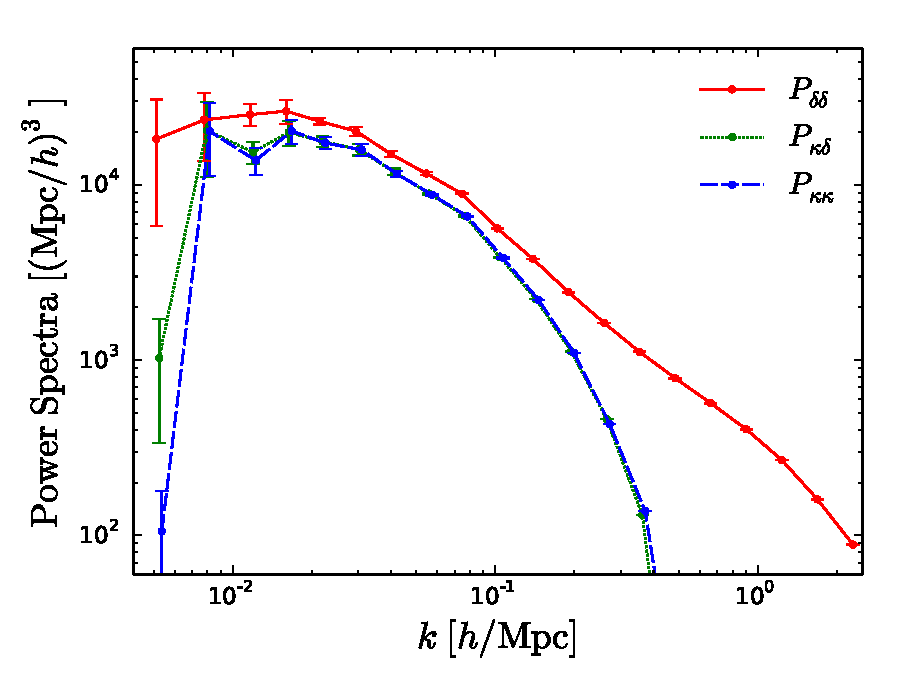
\includegraphics[width=0.48\textwidth]{fig1b.eps}
\end{center}
\vspace{-0.7cm}
\caption{\label{fig:1} Power spectra for different fields. The red solid line
shows the power spectrum of the original density field $\delta(\bm{x})$. 
The green dotted line shows the cross power spectrum of the original density
field and the reconstructed density field $\kappa(\bm{x})$. The blue dashed
line shows the power spectrum of the reconstructed density field 
$\kappa(\bm{x})$.}
\end{figure}

The cross-correlation between the reconstructed field and the original field shows quantitatively how well is 
the reconstruction. In Fig. \ref{fig:1}, we show the auto power spectra of the original field $\delta$, 
the reconstructed field $\kappa$ and the cross power spectrum of the two,
Data points of the three spectra in the same $k$-bin are shifted slightly for clarity of display. 
We see a good cross correlation between the original and the reconstructed 
density fields over a wide range in wave numbers. The power spectrum for $\kappa$
and the cross power spectrum between $\kappa$ and $\delta$ are almost the same.
%Since we apply the Wiener filter $W(k_\parallel,k_\perp)$ to the noisy
%3D convergence field $\kappa_\mr{3D}$, only the part fully correlated with
%the original density field remains in the clean density field $\kappa(\bm{x})$. 
In Fig. \ref{fig:2} we plot the cross correlation coefficient, which is defined as 
$r_{\kappa\delta} \equiv {P_{\kappa\delta}}/{\sqrt{P_{\delta\delta}
P_{\kappa\kappa}}}$. 
%We first average the
%power spectra over the six simulations and then calculate the cross 
%correlation coefficient. 
The error bars are estimated by the Bootstrap resampling method.
For our fiducial case where a smoothing scale of $1.25 \Mpc/h$ is used, 
the correlation coefficient is above 0.8 for $k\lesssim$ 0.1 Mpc/$h$,  and is close to 0.9 at some scales. 

\subsection{Dependence on Smoothing Scale and Gaussianization}
To test how does the reconstruction result depends on the choice of smoothing scale, 
we also performed reconstruction with two more smoothing scales, 
$R=2.5\ \mr{Mpc}/h$ and $R=5\ \mr{Mpc}/h$. 
Fig. \ref{fig:2} shows the cross correlation coefficients
for all these three cases. We see that 
the cross correlation coefficient decreases when the smoothing scales are increased. This 
is expected: the information encoded in the anisotropic small scale structures are used to reconstruct the large scale density field, with large smoothing length, some information 
hidden in the small scale structures are lost, resulting low signal-to-noise ratio in the reconstructed
field. However,  the reconstruction results do not degrade significantly
until the smoothing scale goes beyond $5\ \mr{Mpc}/h$, which is also roughly the scale on which the structure growth transits from linear to non-linear,  so the reconstruction is not sensitive to the smoothing scale unless we smooth on the linear scales. \textcolor{red}{The scale 5 Mpc/h is 
roughly the nonlinear scale, but I am not too sure if this degradation is really due to non-linearity, or it is merely a problem with limited available
modes. Judging from the shape, the latter seems likely. Need to check this, either with analytical formula, or by some kind of test, e.g. in the finer resolution case, only use a fraction of the modes
for reconstruction.}

\begin{figure}[tbp]
\begin{center}
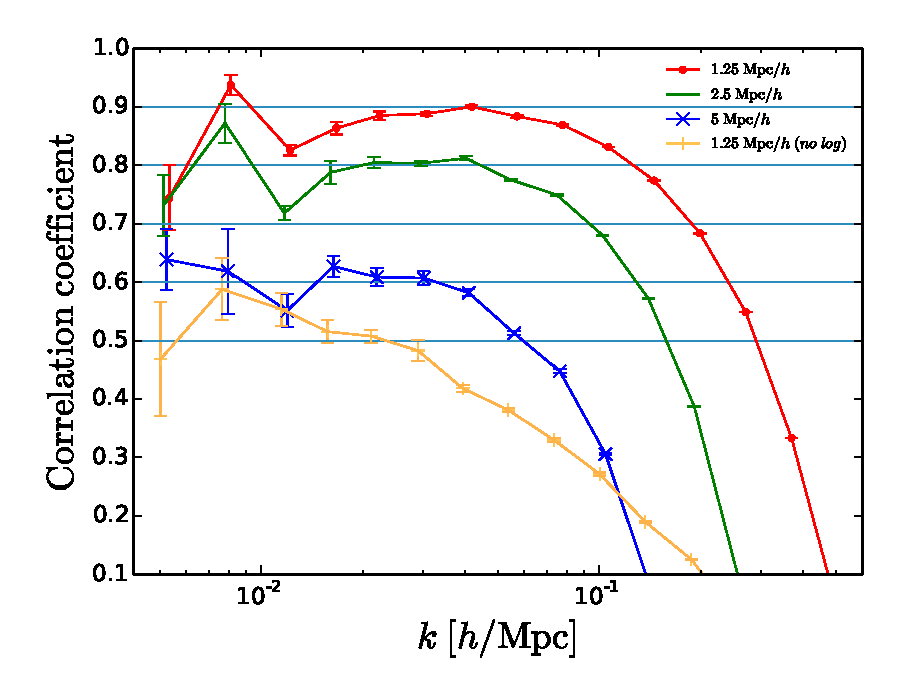
\includegraphics[width=0.48\textwidth]{fig2d.eps}
\end{center}
\vspace{-0.7cm}
\caption{\label{fig:2} Cross correlation coefficients for different 
smoothing lengths and the reconstruction without applying logarithmic transformation.}
\end{figure}

The logarithmic transform plays an important role in cosmic tidal 
reconstruction. In  Figure \ref{fig:2} we also plot the result for a reconstruction 
without the logarithmic transform. We find the cross correlation between the 
reconstructed field and the original field is much weaker than the 
one obtained with logarithmic transformation,  and quickly drops to nearly zero when the wavenumber increases. 
Apparently,  in this case the non-Gaussianity developed in the density field 
impaired the accuracy of the shear reconstruction. The tidal shear
estimators derived with the Gaussian assumption are not necessarily optimal
for the non-Gaussian case. However, the logarithmic transform captures a large part of the 
non-linear evolution, it also fixes the displacement-density relation significantly as shown in 
\cite{2012:log}, so the logarithmic transformation greatly reduces the 
non-Gaussianity of the density field, allowing much better result to be achieved.
%One reason is that the tidal shear estimators is derived under the Gaussian
%assumption \cite{2008:lu}\cite{2010lu}\cite{2012bucher}. 
%The density field itself is non-Gaussian before the logarithmic transformation.
\textcolor{blue}{is this argument good??}

%\begin{figure}[tbp]
%\begin{center}
%\includegraphics[width=0.48\textwidth]{fig3a.eps}
%\end{center}
%\vspace{-0.7cm}
%\caption{\label{fig:3} Cross correlation coefficients with and without
%gaussianization. The cross correlation is signigicantly weaker when we
%reconstruct without gaussianization.}
%\end{figure}

\subsection{The Anisotropic Noise}
For the reconstruction described above, the error in $\kappa_\mr{3D}$ is anisotropic as we 
discussed earlier. We show the anisotropic noise power spectrum in Fig. \ref{fig:noise}. 
The noises for modes with large $k_\parallel$ and small $k_\perp$ are orders of
magnitude larger than other modes. This result confirms the estimate of noise derived from 
theory, $\sigma_{\kappa_\mr{3D}}\propto k^2/k_\perp^2$, which diverges for
small $k_\perp$. In Fig. \ref{fig:ratio}, we show the anisotropic correlation coefficient
$r_{\kappa\delta}(k_\parallel,k_\perp)=P_{\kappa\delta}(k_\parallel,k_\perp)/\sqrt{
P_{\delta\delta}(k_\parallel,k_\perp)P_{\kappa\kappa}(k_\parallel,k_\perp)}$.
The correlation between the original and the reconstructed field is better 
at the lower right corner, which could be close to 1 for modes with large $k_\perp$, but drops
to 0 quickly when $k_\parallel$ increases, the modes with large $k_\parallel$ 
and small $k_\perp$ are poorly reconstructed.

%Figure \ref{fig:wf} shows the 
%Wiener filter $W(k_\parallel,k_\perp)$. 
%$W(k_\parallel,k_\perp)$ is close to 1 at the lower right corner and drops to 0
%at the upper left corner.
%Hence those modes with large $k_\parallel$ and small $k_\perp$ contain 
%nothing but noise.
In Fig. \ref{fig:bias} we show the anisotropic bias factor, which
is almost scale independent, except for modes with very large $k_\parallel$ and 
very small $k_\perp$, where the cosmic tidal reconstruction failed. 


Such anisotropy in reconstruction is due to the fact we only use tidal shear fields in
the $x-y$ plane to reconstructed the long wavelength  density field.
The changes of the long wavelength density field $\delta_L$ are inferred from the 
variation of tidal shear fields $\gamma_+(\bm{x})$ and $\gamma_\times(\bm{x})$ 
along $z$ axis, i.e. we reconstruct these modes indirectly, so we can not
capture rapid changes of the density field along $z$ axis. 
By including tidal shear fields containing
derivatives with respect to $z$ axis, the reconstruction may be improved. 
However, accurate radial direction measurement requires more observing resources,
and in any case redshift space distortion will inevitably affect the reconstruction result. 
We leave the detailed study of this  in  a future paper.

\begin{figure}[tbp]
\begin{center}
\includegraphics[width=0.48\textwidth]{f3.eps}
\end{center}
\vspace{-0.7cm}
\caption{\label{fig:noise} The anisotropic noise power spectrum $P_n(k_\parallel, k_\perp)$.
}
 \end{figure}

\begin{figure}[tbp]
\begin{center}
\includegraphics[width=0.48\textwidth]{f4.eps}
\end{center}
\vspace{-0.7cm}
\caption{\label{fig:ratio} The anisotropic cross correlation coefficient 
$r_{\kappa\delta}(k_\parallel,k_\perp)$.
}
 \end{figure}

%\begin{figure}[tbp]
%\begin{center}
%\includegraphics[width=0.48\textwidth]{f5.eps}
%\end{center}
%\vspace{-0.7cm}
%\caption{\label{fig:wf} 2D Wiener filter $W(k_\parallel,k_\perp)$. The Wiener
%fielter is close to 1 when $k_\perp$ is large and $k_\parallel$ is small.
%It drops to zero quickly when $k_\perp$ is small and $k_\parallel$ is large,
%since these reconstructed modes are noisy.}
% \end{figure}

\section{Discussions}
In this paper we studied the tidal distortions of long wavelength perturbations on 
the small scale perturbations, and showed how the long wavelength perturbation can 
be reconstructed from the small scale anisotropic perturbations. 
We considered the tidal distortions  which are
 proportional to $\hat{k}^i\hat{k}^jt_{ij}^{(0)}$, and assumed that the
proportional coefficient varies slowly over different wave numbers.
We can absorb the unknown coefficient into the bias factor introduced
in Eq.(\ref{eq:kap3d}), then measure it  with $N$-body 
simulations. The proportional constant from the Poisson equation \textcolor{red}{which?}
and the normalization constant $Q$ in the tidal shear estimators can also be absorbed
in this bias factor. 
The integral for $Q$ in Eq.(\ref{eq:Q}) would diverge at large $k$ if
there were no noise in the power spectrum $P(k)$, i.e. $P(k)=P_{tot}(k)$, 
as happens when we use the 
dark matter density field from high precision $N$-body simulations to
reconstruct the large scale density field. The bias factor solves 
this problem.\textcolor{red}{I am a bit confused by this point, more explanation? Also, 
this discussion can be put right after Eq.(\ref{eq:Q}) }.


Here we considered the leading order effect, i.e. the coupling between $\mb{s}_{1s}$ and $\mb{s}_{1t}$. 
 Higher order terms of the form $(\mb{s}_{1s})^n\mb{s}_{1t}$  with $(n>1)$ may also make 
significant contribution,  as the nonlinearities on small scales are quite strong. 
The proportional coefficient $f(k,\tau)$ in Eq.(\ref{eq26}) will be changed  if such higher
order terms are included. The result could be improved in the future by including the higher 
order perturbations. Nevertheless, 
he reconstruction is well performed , with the cross correlation coefficient larger than 0.8
until $k\gtrsim0.1\mr{Mpc}/h$ and on some scales close to 0.9.
The reconstruction should work even better
at higher redshifts where  the small scale density
fluctuations undergo less nonlinear evolution. 


\begin{figure}[tbp]
\begin{center}
\includegraphics[width=0.48\textwidth]{f6.eps}
\end{center}
\vspace{-0.7cm}
\caption{\label{fig:bias} 2D bias factor $b(k_\parallel,k_\perp)$. The bias 
factor is almost scale independent in this plane. 
$b(k_\parallel,k_\perp)$ saturates at the upper left corner. Since these
modes are noisy, the extremely large values of the bias at that corner are 
not reliable.}
\end{figure}

The $\hat{\gamma}_+$ and $\hat{\gamma}_\times$ estimators are unbiased
and of minimum variance in the long wavelength limit, providing optimal tidal
shear reconstructions. However, at larger wavenumbers, the tidal shear fields would be underestimated
by a scale dependent bias factor which need to be corrected.
The estimator derived in the long wavelength limit 
still works well if we only use the reconstruction modes with scale larger than 
the smoothing scale. However, when there is an overlap between these two scales, the reconstruction 
result would degrade. More sophisticated method is needed in that case.  Also, 
the estimators we derived in this paper are optimal under the Gaussian assumption, but in reality
the nonlinear density field is not  Gaussian. The logarithmic transformation helps to  Gaussianize the non-Gaussian
density field and as a result we still get pretty good result. It would be worthwhile to investigate the 
 optimal estimators for non-Gaussian sources, which can be constructed from $N$-body
simulations.  Finally,  here we use the dark matter density field directly to reconstructed the large scale 
density field. However, galaxies and halos are distributed in the 
underlying dark matter density field. Due to the discreteness of the 
galaxy/halo field, the tidal reconstruction
may not be as good as that of the dark matter field. The scale dependent 
galaxy/halo bias may also complicate the reconstruction. We plan to study this in future.



The reconstruction method developed in this paper has many applications. 
For example, the reconstructed field $\kappa$ gives the distribution of dark matter
on large scales, by cross correlating with the original galaxy/halo field,
we could measure the logrithmic growth rate without sample variance 
\cite{2009mcdonald}. This potentially gives precision measurements of neutrino
masses and tests of gravity. Moreover, it can also be applied to the case where 
the measurement of longwave mode is missing, for example the 
 data obtained with the 21cm intensity mapping survey.
In 21cm intensity mapping surveys, modes with small radial wavenumber is contaminated 
by foreground radiation and is often subtracted in data analysis,
which makes it impossible to do cross-correlation with surveys which provide only 
long mode measurement, such as the measurements made with weak lensing tomography, 
photo-$z$ galaxies, integrated Sachs-Wolf effect and kinematic Sunyaev Zel'dovich effect.
Since cosmic tidal reconstruction can recover these long wavelength modes from small 
scale modes, it would enable us to reconstruct the long wavelength modes from 21cm intensity mapping data, 
which can be used to  cross correlate with the other cosmic probes. This is be investigated in 
another paper \textcolor{red}{But there are some problems in this arguement. The method given here would 
be useful in reconstructing density modes, but not useful to reconstruct 21cm modes. The 21cm modes also 
include the effect of ionization fraction and spin temperature, which can not be recovered from this reconstruction.
When people do the cross-correlation they are usally trying to look for these effects, not the density modes.} 



%From 21cm intensity mapping surveys, we get a 3D temperature field.
%Both tidal interaction and gravitational lensing will distort the apparent
%temperature field. However, the distortion from tidal interaction is due to the 
%long wavelength tidal field and the distrotion from weak lensing is due to the 
%projected foreground density field.
%The slight difference is that the foreground density field only remaps the 
%original temperature field  without changing the temperature field itself.
%While the large scale tidal field not only affects the displacement of 
%particles in the small dark matter fluid, but also effects the evolution of 
%small scale density fluctuations.

Finally, the tidal reconstruction will be useful in the study of 21cm lensing, where distant 
21cm signal are used as the source for lensing.  The nonlinearity in the 21cm temperature 
field limits the precision of lensing reconstruction  \cite{2008:lu,2010lu}. 
However, the tidal interaction is also responsible for the local quadrupole distortions,
so we could use the large scale density to remove the tidal distortions to 
reduce the nonlinarities in the observed 21cm temperature field, just like BAO
reconstruction. This will improve 21cm lensing significantly. 



\section{Acknowledgement}
We acknowledge the support of the Chinese MoST 863 program under Grant 
No. 2012AA121701, the CAS Science Strategic Priority Research Program 
XDB09000000, the NSFC under Grant No. 11373030, Tsinghua University, 
CHEP at Peking University, and NSERC. 
X. Er is supported by the NSFC under Grant No. 11473032.

\bibliographystyle{apsrev}
\bibliography{tide}
\end{document}
